The database was designed in a way that reduces redundant information to a
minimum. The structure diagram is shown in Figure \ref{fig:dbstructure} (page
\pageref{fig:dbstructure}). All tables except the ``ests'', ``hmmsearch'', and
``blast'' tables are used to store information about the amino acid or
nucleotide sequences that belong to either an ortholog set or a proteome of a
core taxon, or both. 

All tables have an ``id'' column with an auto-incremented integer as a unique
identifier. Normally, this identifier is used in \code{JOIN} queries that
reference other tables.

The tables ``aaseqs'' and ``ntseqs'' are filled with the peptide or
nucleotide sequences, respectively, that belong to the ortholog sets. One or
both are referenced to a sequence pair in the table ``sequence\_pairs''. 

The table ``set\_details'' contains a shorthand name for each ortholog set along
with its longer name or description. 

At the time of this writing, the tables ``ests'', ``hmmsearch'' and ``blast''
are filled in a cumulative fashion, i.e., they contain data from all query
species. This affects performance because without administrative access to
server configuration and tuning variables, a too small InnoDB key buffer along
with very large tables becomes a performance bottleneck \citep{mysql2013}. Also
for this reason, and because


% this is probably not that useful
%\input{inc/results/tab-mysql-variables}

\begin{figure}[h!]
	\centering
	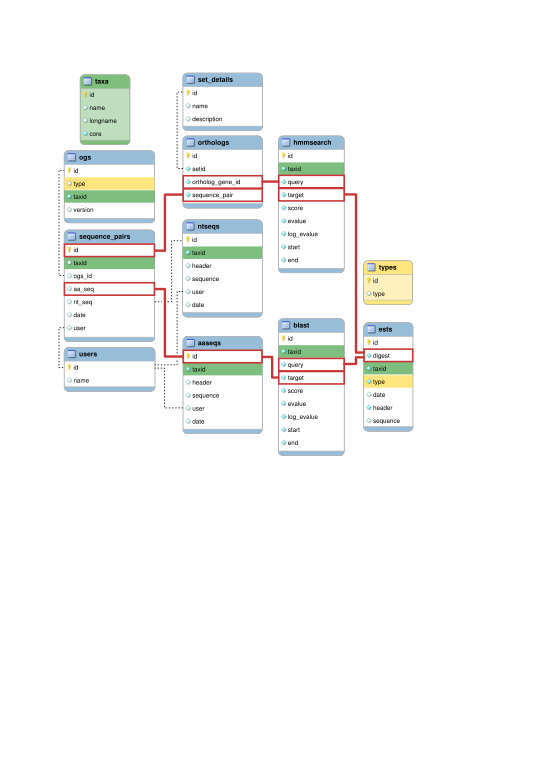
\includegraphics[width=\textwidth]{img/dbstructure.pdf}
	\caption[Complete \pname database structure]{
		\pname database structure. Each rounded rectangle represents a table with
		named columns. Note the circular path (red) that can be drawn across the
		tables and that is used in queries across multiple tables in order to
		construct a graph of orthologous relationships. Green table columns are
		referenced to the ``taxa'' table, and yellow table columns are referenced to
		the ``types'' table. Dotted lines are secondary references that provide
		additional information for individual records.
	}
	\label{fig:dbstructure}
\end{figure}



